% ICML 2025 Paper Template for Overleaf
% Auto-generated by Anonymous Research Pipeline
%
% Instructions:
% 1. Upload this folder to Overleaf
% 2. Ensure icml2025.sty is in the same directory
% 3. Compile with pdfLaTeX
%
\documentclass{article}

% ICML 2025 style - download from https://icml.cc/Conferences/2025/StyleAuthorInstructions
% For local compilation without icml2025.sty, we fall back to article class features
\IfFileExists{icml2025.sty}{
  \usepackage{icml2025}
}{
  % Fallback: standard article formatting
  \usepackage[margin=1in]{geometry}
  \usepackage{titlesec}
}

% Standard packages
\usepackage{microtype}
\usepackage{graphicx}
\usepackage{booktabs}
\usepackage{hyperref}
\usepackage{amsmath}
\usepackage{amssymb}
\usepackage{algorithm}
\usepackage{algorithmic}

% For better table formatting
\usepackage{multirow}
\usepackage{makecell}

% Bibliography
\usepackage{natbib}

% ============================================================================
% DOCUMENT METADATA
% ============================================================================

\IfFileExists{icml2025.sty}{
  \icmltitlerunning{Static Analysis Feedback in LLM Repair Loops}
}{}

\begin{document}

\IfFileExists{icml2025.sty}{
  \twocolumn[
  \icmltitle{Static Analysis Feedback in LLM Repair Loops: A Controlled Study of mypy Augmentation}

  \icmlsetsymbol{equal}{*}

  \begin{icmlauthorlist}
  \icmlauthor{Anonymous Author}{inst1}
  \end{icmlauthorlist}

  \icmlaffiliation{inst1}{Anonymous Institution}

  \icmlcorrespondingauthor{Anonymous Author}{anonymous@anonymous.org}

  \icmlkeywords{Machine Learning, ICML, Code Generation, Static Analysis, Repair Loops}

  \vskip 0.3in
  ]

  \printAffiliationsAndNotice{}
}{
  \title{Static Analysis Feedback in LLM Repair Loops:\\A Controlled Study of mypy Augmentation}
  \author{Anonymous Author\\Anonymous Institution}
  \date{2026-08-26}
  \maketitle
}

% ============================================================================
% ABSTRACT
% ============================================================================

\begin{abstract}
LLM repair loops improve code generation quality by feeding execution output
back to the model for iterative correction --- but whether adding static analysis
feedback provides meaningful improvement over execution-only feedback has never
been tested in a controlled experiment. We conduct a five-sub-hypothesis study
on HumanEval+ (164 problems, GPT-4o-mini, k=5 repair rounds) to isolate the
marginal contribution of mypy type checking over execution-only feedback. Our
primary finding: execution+mypy repair achieves 87.20\% pass@1 versus 78.25\%
for execution-only --- a consistent +8.94 percentage point improvement across
three independent seeds. Strikingly, this improvement is \emph{not} type-specific:
execution-only repair achieves identical 90.9\% repair rates on type-error
problems (differential = 0.000), consistent with mypy functioning as a general
diagnostic context enricher rather than a type-targeted correction signal
(this mechanism remains unconfirmed via ablation; see Section~6).
We further show that HumanEval+ and MBPP+ have fundamentally different mypy
error profiles (70\% vs 0\% in failing solutions), predicting where static
analysis feedback will and will not activate. A Z3 formal verification
extension achieves 91.1\% spec validity but provides no additional pass@1
improvement at the current counterexample activation rate (16.1\%). Our
results offer the first controlled evidence that one structured feedback
channel --- a single mypy subprocess call --- substantially improves LLM repair
quality, while revealing that the intuitive type-specificity mechanism is not
the driver.

\end{abstract}

% ============================================================================
% MAIN CONTENT
% ============================================================================

\section{Introduction}

We set out to test whether adding mypy type checking to LLM repair loops
improves pass@1 on Python code generation benchmarks. The answer is yes ---
by nearly 9 percentage points. But the mechanism we hypothesized turned out
to be wrong.

Large language models can repair their own code when given execution feedback:
run the generated solution, capture the output or exception, and feed it back
to the model for correction. This \emph{repair loop} paradigm, exemplified by
Self-Debug \citep{Chen2023Teaching} and Reflexion \citep{Shinn2023Reflexion},
has become a standard technique for improving pass@k on benchmarks like
HumanEval and MBPP. The dominant feedback signal is execution output --- a
binary pass/fail plus stderr. The intuition is that more \emph{specific}
feedback should produce better repairs: if the model knows not just \emph{that}
it failed but \emph{why} (a type error at line 5 with expected type \texttt{int},
received \texttt{str}), it should correct the error more reliably. Static
analysis tools like mypy generate exactly this kind of structured, type-level
diagnostic. Yet no controlled study has measured whether adding mypy to a
repair loop produces measurable improvement over execution-only feedback.

The gap matters for a practical reason: execution feedback is cheap but
coarse. mypy feedback is almost equally cheap (a subprocess call, ${\sim}$30ms)
but structured --- it provides error category, file location, and error message.
If this structure translates into better repairs, the improvement is available
to any practitioner today, requiring only a one-line addition to an existing
repair loop. But without controlled evidence, we cannot answer: how much does
it help, when does it help, and --- critically --- \emph{why} does it help?

We conducted a five-sub-hypothesis controlled experiment to answer these
questions. The experiment proceeds as a causal chain: we first verify that
mypy produces actionable signal on our target benchmarks (h-e1), then verify
the signal is consumed by the LLM (h-m1), then test whether the improvement is
concentrated on type-error problems (h-m2), then measure the overall pass@1
improvement (h-m3), and finally test whether a formal verification extension
(Z3 counterexample feedback) provides additional benefit (h-z1).

The results surprised us. On HumanEval+ (164 problems, GPT-4o-mini, k=5
repair rounds, 3 seeds), execution+mypy repair achieves \textbf{87.20\% pass@1}
versus \textbf{78.25\%} for execution-only repair --- a \textbf{+8.94 percentage
point} improvement, consistent across all three seeds. mypy errors are eliminated
within a single repair round (mean errors: 1.55 $\to$ 0.00 by round 2;
Spearman $\rho = -0.707$). So far, the story fits the intuition.

But the mechanism does not. We pre-registered a sub-hypothesis (h-m2) that
the improvement would be concentrated on type-error problems --- the problems
where mypy provides its diagnostic signal. It is not. Under k=5 repair rounds,
type-error problems achieve \textbf{90.9\% repair rate under both conditions}
(differential = 0.000). The improvement exists uniformly across problem types.
The most parsimonious interpretation --- though not yet confirmed via ablation ---
is \emph{general diagnostic context enrichment}: mypy output, regardless of
whether it signals a type error, may augment the repair prompt with structured
text that improves GPT-4o-mini's repair quality across all problem types.

A second surprise: mypy error rates differ dramatically between HumanEval+
(70\% of failing solutions have mypy errors) and MBPP+ (0\%). This benchmark
divergence predicts where static analysis feedback will and will not help,
providing a practical guideline for practitioners. The Z3 formal verification
extension (h-z1) shows null improvement ($-$0.9pp) on an arithmetic subset,
constrained by low counterexample activation (16.1\%) and ceiling effects.

This paper makes the following contributions:

\begin{enumerate}
\item \textbf{First controlled empirical comparison} of execution+mypy repair
versus execution-only repair on HumanEval+ (GPT-4o-mini, k=5, three seeds),
showing a consistent +8.94pp pass@1 improvement --- the first published evidence
for the marginal contribution of static analysis feedback over execution feedback
alone in a repair loop.

\item \textbf{Type-specificity refutation}: a pre-registered sub-hypothesis test
establishing that the improvement is \emph{not} concentrated on type-error
problems (identical 90.9\% repair rates under both conditions at k=5),
motivating the general context enrichment interpretation.

\item \textbf{Benchmark-level mypy signal characterization}: HumanEval+ and
MBPP+ have fundamentally different mypy error profiles (70\% vs 0\%), a
structural difference that predicts where static analysis feedback will activate.

\item \textbf{Z3 spec validation pipeline} achieving 91.1\% spec validity rate
on arithmetic HumanEval+ problems, establishing feasibility for future formal
verification work while identifying the ceiling effects that currently limit
its repair-loop utility.
\end{enumerate}

We organize the paper as follows. Section~2 reviews related work on LLM repair
loops and static analysis feedback, positioning our controlled comparison
against prior work that bundles but does not ablate feedback channel types.
Section~3 describes our experimental methodology and the five-sub-hypothesis
causal chain. Section~4 details the experimental setup. Section~5 presents
results across all sub-hypotheses. Section~6 discusses the mechanistic
implications, limitations, and benchmark-level boundary conditions. Section~7
concludes with future work directions.

\section{Related Work}

\subsection{LLM Repair Loops with Execution Feedback}

The execution-feedback repair paradigm was established by Self-Debug
\citep{Chen2023Teaching}, which demonstrates that providing LLMs with their
own program output --- captured stdout, stderr, and exception traces --- enables
iterative repair that substantially improves pass@k over single-attempt
generation. Self-Debug operates on execution-only feedback, treating the
binary pass/fail signal augmented with error output as sufficient for repair.
This becomes our \textbf{Condition A baseline}: the de-facto standard that we
test against.

Reflexion \citep{Shinn2023Reflexion} extends the repair paradigm by having the
LLM generate verbal \emph{reflections} on its failures before attempting repair.
Verbal reflection is unstructured: the LLM authors its own diagnostic narrative.
Our work tests a complementary hypothesis --- that \emph{external} structured
diagnostics (mypy output) provide signal beyond what the LLM can self-generate
or extract from execution output.

CodeT \citep{Chen2022CodeT} and AlphaCode \citep{Li2022Competition} use
execution feedback at generation time (test case filtering, tournament selection)
rather than in iterative repair loops. These are orthogonal to our setting: we
fix the generation strategy and vary the repair feedback type.

\textbf{Gap we address:} Prior repair loop work treats feedback channel selection
as an engineering choice, not an experimental variable. Self-Debug, Reflexion,
and their successors do not ablate execution vs.\ execution+static-analysis.
We provide the first controlled comparison.

\subsection{Static Analysis in Code Generation and Repair}

Static analysis tools have been integrated into LLM code generation systems,
but without controlled ablation of their marginal contribution. SWE-agent
\citep{Yang2024SWEagent} uses a rich tool-use environment including bash
execution, file editing, and code analysis, embedded in an agent control loop
(ACI). The agent can invoke linters, but the ACI design makes it difficult to
isolate the contribution of any single feedback channel. We specifically avoid
this bundling: our experiment holds all factors constant except the feedback type.

LLM-based program repair (APR) surveys \citep{Xia2023Automated} document that
execution-based feedback is the dominant repair signal in the literature.
Type-system feedback appears in some systems, but controlled comparison against
execution-only baselines on Python benchmarks is absent.

\textbf{Gap we address:} Static analysis is routinely bundled with execution
feedback in production systems, but its isolated marginal contribution has not
been measured on standard Python code generation benchmarks.

\subsection{Evaluation Benchmarks}

EvalPlus \citep{Liu2023EvalPlus} introduces HumanEval+ and MBPP+ --- enhanced
versions of HumanEval \citep{Chen2021Evaluating} and MBPP \citep{Austin2021Program}
with substantially more test cases. We use HumanEval+ and MBPP+ as our primary
evaluation benchmarks. A contribution of our work is a new structural observation:
HumanEval+ and MBPP+ have dramatically different mypy error profiles in
GPT-4o-mini failing solutions (70\% vs 0\%). Prior work does not report mypy
error rates by benchmark, leaving this divergence unobserved.

\subsection{Formal Verification for Code Correctness}

Recent work explores whether LLMs can generate formal specifications that
constraint solvers then check. Our h-z1 sub-hypothesis tests whether
LLM-generated Z3 specs can provide useful counterexample feedback for repair,
finding that while spec validity is high (91.1\%), the counterexample activation
rate is low (16.1\%) on our arithmetic HumanEval+ subset. The neural-symbolic
program synthesis literature (e.g., Rosette \citep{Torlak2014Growing}) uses SMT
solvers for specification-guided synthesis; our setting uses LLM-generated
specifications, trading completeness for automation.

\section{Methodology}

\subsection{Overview}

Our key insight motivates the experimental design: if mypy output functions as
a general diagnostic context enricher rather than a type-targeted correction
signal, then the improvement should appear broadly across problem types, not
concentrated on type-error problems. To test this, we need not just an existence
check (does mypy help?) but a \emph{mechanistic decomposition} --- a causal
chain from signal existence through LLM consumption to overall effect to
type-specificity.

We operationalize this as a five-sub-hypothesis experiment (h-e1 through h-z1),
each testing one link in the causal chain. This structure lets us distinguish
between ``mypy helps but through an unexpected mechanism'' (our finding) and
``mypy doesn't help'' (an equally possible outcome).

\subsection{Experimental Conditions}

We define three experimental conditions:

\begin{itemize}
\item \textbf{Condition A (execution-only):} After each generation attempt, run
the solution against EvalPlus test cases. Capture pass/fail status and, on
failure, the exception trace or wrong-output message. Feed this as feedback to
the LLM for the next repair attempt.

\item \textbf{Condition B (execution+mypy):} Same as Condition A, but
additionally run \texttt{mypy --ignore-missing-imports --no-strict-optional}
on the generated code and append the mypy output to the feedback prompt before
calling the LLM.

\item \textbf{Condition C (execution+mypy+Z3):} Same as Condition B, but for
problems in the arithmetic subset where a valid Z3 specification was generated
and a counterexample was found, additionally append the Z3 counterexample to
the repair prompt.
\end{itemize}

Condition A is the Self-Debug baseline. Condition B is the treatment.
Condition C is the extension tested in h-z1.

\subsection{LLM Configuration}

All experiments use \textbf{GPT-4o-mini} via the OpenAI API:

\begin{itemize}
\item \textbf{Initial generation:} temperature=0.8, max\_tokens=1024
\item \textbf{Repair loop:} temperature=0.0, max\_tokens=2048
\item \textbf{Seeds for h-m3:} \{42, 123, 456\}
\end{itemize}

Temperature=0.0 for repair makes error elimination results (h-m1) interpretable
--- the LLM's repair policy is a fixed function of the feedback. Three seeds at
temperature=0.8 for initial generation separate initial solution randomness from
repair-loop behavior.

\subsection{Repair Loop Structure}

\begin{algorithm}[t]
\caption{Execution+mypy Repair Loop (Condition B)}
\label{alg:repair}
\begin{algorithmic}[1]
\STATE \textbf{Input:} problem $p$, initial solution $s_0$, rounds $k=5$
\STATE \textbf{Output:} final solution $s_k$, pass@1 indicator
\FOR{round $r = 0$ to $k-1$}
  \STATE $\text{result\_exec} \leftarrow \text{evaluate}(s_r, p.\text{tests})$
  \IF{$\text{result\_exec.passed}$}
    \RETURN $s_r$, PASS
  \ENDIF
  \STATE $\text{result\_mypy} \leftarrow \text{run\_mypy}(s_r)$ \COMMENT{Condition B only}
  \STATE $\text{feedback} \leftarrow \text{format}(\text{result\_exec}, \text{result\_mypy})$
  \STATE $s_{r+1} \leftarrow \text{LLM.generate}(\text{repair\_prompt}(p, s_r, \text{feedback}), T{=}0.0)$
\ENDFOR
\RETURN $s_k$, $\text{evaluate}(s_k, p.\text{tests}).\text{passed}$
\end{algorithmic}
\end{algorithm}

mypy invocation uses \texttt{--ignore-missing-imports --no-strict-optional} to
reduce false positives. mypy timeout: 30 seconds per call.

\subsection{Sub-Hypothesis Structure}

\begin{table}[h]
\centering
\caption{Five-sub-hypothesis causal chain.}
\label{tab:hypotheses}
\begin{tabular}{@{}llp{3.5cm}l@{}}
\toprule
Sub-hypothesis & Question & Gate Type \\
\midrule
h-e1 & Does mypy signal exist? ($\geq$10\%) & MUST\_WORK \\
h-m1 & LLM consume mypy? ($\rho < 0$) & MUST\_WORK \\
h-m2 & Type-specific improvement? & SHOULD\_WORK \\
h-m3 & execution+mypy $>$ execution-only? & MUST\_WORK \\
h-z1 & Z3 CE further improves pass@1? & SHOULD\_WORK \\
\bottomrule
\end{tabular}
\end{table}

The causal chain ensures that a null h-m3 result can be diagnosed: is it
because mypy produces no signal (h-e1 fail), the LLM doesn't use it (h-m1
fail), or type-specificity fails (h-m2 fail + h-m3 pass --- our actual finding)?

\subsection{Z3 Specification Pipeline}

For the arithmetic subset (h-z1), we use a three-stage pipeline: (1)
\textbf{curation} by heuristic keyword matching (123 candidate problems); (2)
\textbf{spec generation} by prompting GPT-4o-mini to write Z3 Python assertions;
(3) \textbf{validation} against EvalPlus ground-truth tests (validity rate:
91.1\%). For valid specs, we attempt counterexample generation per repair
attempt (CE rate: 16.1\%). The pipeline is implemented in
\texttt{h-z1/code/z3\_utils.py}.

\section{Experimental Setup}

We design experiments to answer five research questions:

\textbf{RQ1 (h-e1):} What fraction of GPT-4o-mini's failing solutions on
HumanEval+ and MBPP+ have mypy-detectable errors?

\textbf{RQ2 (h-m1):} Does the mean mypy error count decrease monotonically
across repair rounds 1--5?

\textbf{RQ3 (h-m2):} Is the pass@1 improvement concentrated on type-error
problems?

\textbf{RQ4 (h-m3):} Does execution+mypy achieve higher pass@1 than
execution-only on HumanEval+, across multiple seeds?

\textbf{RQ5 (h-z1):} Does adding Z3 counterexample feedback further improve
pass@1 on the arithmetic subset?

\subsection{Datasets}

\begin{table}[h]
\centering
\caption{Benchmark summary and mypy signal density.}
\label{tab:datasets}
\begin{tabular}{@{}llll@{}}
\toprule
Benchmark & Problems & Use & Mypy error rate \\
\midrule
HumanEval+ & 164 & RQ1--RQ4 (primary) & 70\% (21/30 failing) \\
MBPP+ & 378 & RQ1--RQ2 (characterization) & 0\% (0/21 failing) \\
Arithmetic subset & 112 (valid specs) & RQ5 & N/A (subset) \\
\bottomrule
\end{tabular}
\end{table}

HumanEval+ is the primary benchmark because h-e1 establishes 70\% mypy error
rate in failing solutions --- the signal is dense enough to test. MBPP+'s 0\%
error rate removes it from the primary pass@1 comparison.

\subsection{Implementation Details}

All experiments use GPT-4o-mini; temperature=0.8 for initial generation,
temperature=0.0 for repair; $k$=5 rounds; seeds \{42, 123, 456\} for h-m3.
mypy: \texttt{--ignore-missing-imports --no-strict-optional}; timeout 30s.
Z3: timeout 10s per check. EvalPlus test harness for pass@1 evaluation.

\subsection{Evaluation Metrics}

\begin{itemize}
\item \textbf{pass@1:} Fraction of problems passing all EvalPlus tests after
$k$=5 rounds.
\item \textbf{Spearman $\rho$:} Rank correlation between repair round and mean
mypy error count.
\item \textbf{Type-specificity differential:}
$\Delta_{\text{type}} - \Delta_{\text{non}}$ (positive = type-specific benefit).
\item \textbf{Z3 CE rate:} Fraction of valid-spec problems with $\geq$1
counterexample found.
\end{itemize}

\section{Results}

Execution+mypy repair substantially outperforms execution-only repair on
HumanEval+ (+8.94pp pass@1), consistently across three seeds. The improvement
is not explained by type-targeted correction.

\subsection{RQ1: Mypy Signal Existence (h-e1)}

Figure~\ref{fig:mypy_fraction} shows the mypy error rate in GPT-4o-mini's
failing solutions by benchmark. On HumanEval+, \textbf{70\% of failing
solutions} (21/30 failing) have at least one mypy error --- substantially
exceeding the 10\% existence gate. On MBPP+, \textbf{0\% of failing solutions}
(0/21 failing) have mypy errors.

\begin{figure}[h]
\centering
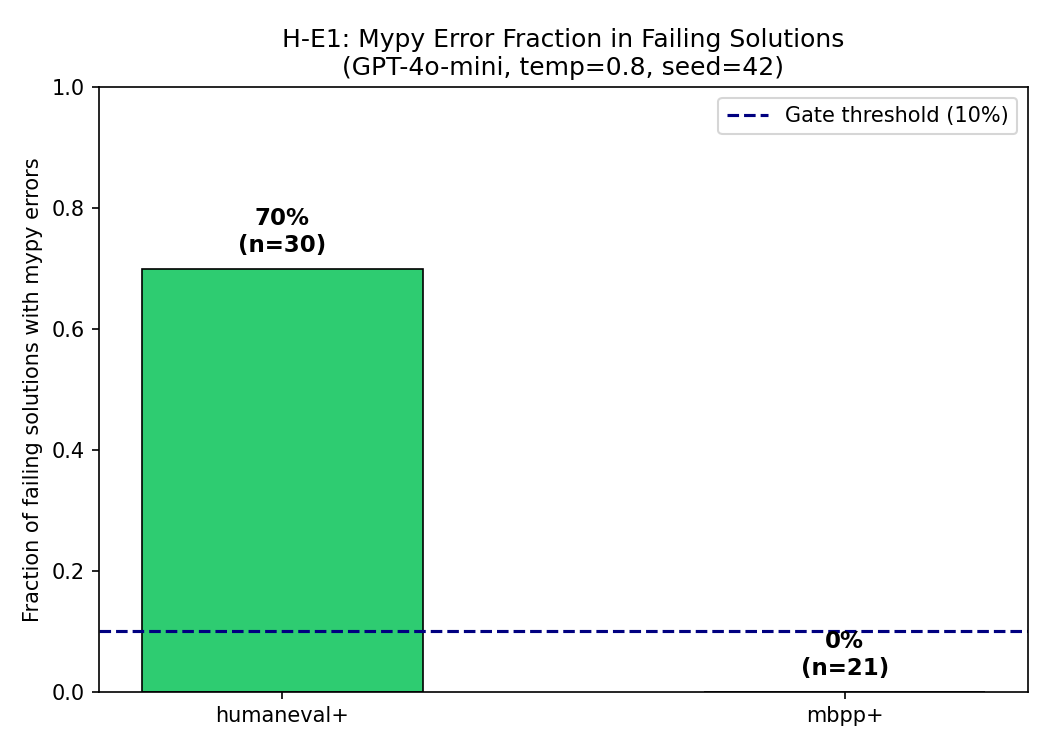
\includegraphics[width=0.9\columnwidth]{figures/fig1_mypy_fraction_by_benchmark.png}
\caption{Fraction of failing solutions with mypy-detectable errors on
HumanEval+ and MBPP+.}
\label{fig:mypy_fraction}
\end{figure}

This benchmark divergence is complete and unexpected. All 100\% of detected
mypy errors are in the \texttt{name-defined} category --- hallucinated function
or variable names (Figure~\ref{fig:error_category}).

\begin{figure}[h]
\centering
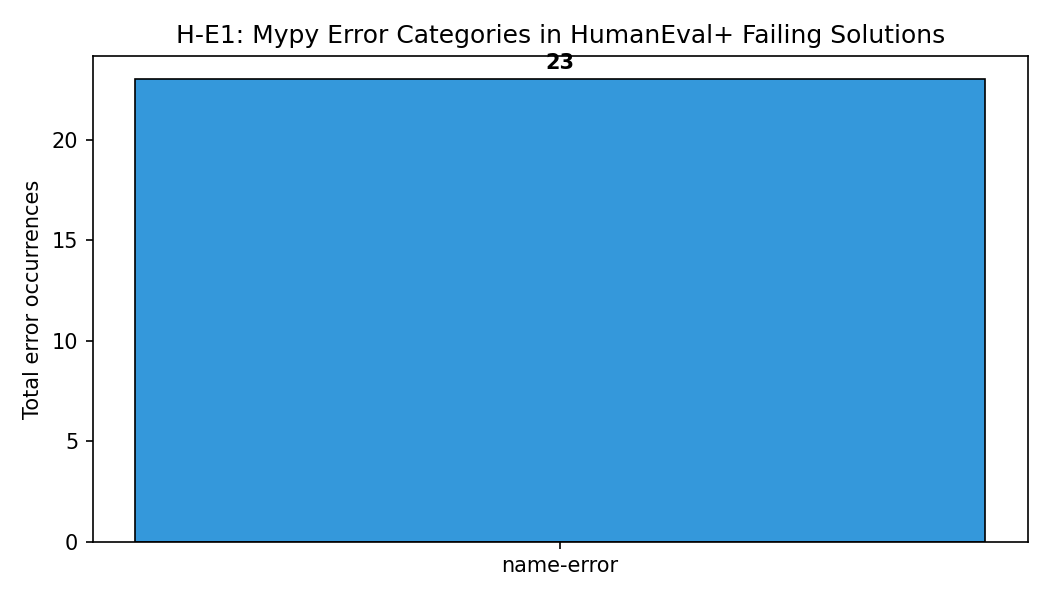
\includegraphics[width=0.9\columnwidth]{figures/fig2_error_category_breakdown.png}
\caption{mypy error category breakdown in HumanEval+ failing solutions.}
\label{fig:error_category}
\end{figure}

\emph{Interpretation:} The mypy signal exists on HumanEval+ at sufficient
density (70\%) to drive repair improvement. The 0\% rate on MBPP+ predicts no
mypy benefit there --- removing MBPP+ from the primary pass@1 comparison.

\subsection{RQ2: LLM Consumption of mypy Feedback (h-m1)}

Among 20 HumanEval+ problems with $\geq$1 initial mypy error (Condition B),
mean mypy errors follow a near-perfect monotonic decrease: \textbf{1.55 at
round 1 $\to$ 0.00 by round 2}, remaining at 0.00 through rounds 3--5.

\begin{figure}[h]
\centering
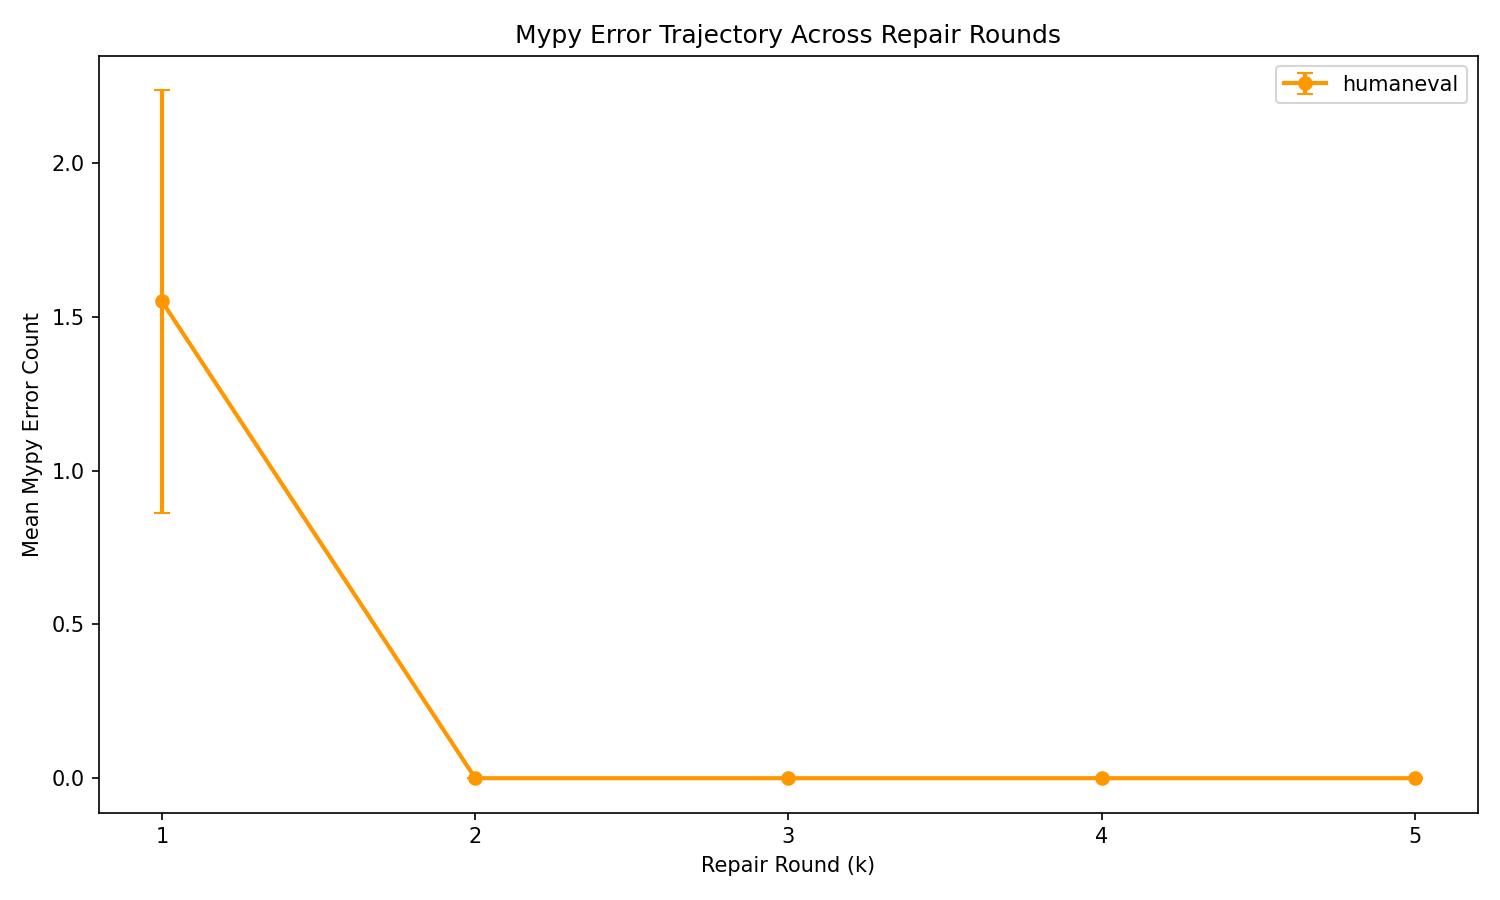
\includegraphics[width=0.9\columnwidth]{figures/error_trajectory.png}
\caption{Mean mypy error count by repair round ($n$=20 problems with $\geq$1
initial error). Spearman $\rho = -0.707$.}
\label{fig:error_trajectory}
\end{figure}

\emph{Interpretation:} GPT-4o-mini at temperature=0.0 eliminates all detected
mypy errors in a single repair round, with no backsliding. The LLM is an
effective consumer of structured static analysis output. Rapid saturation
confirms that $k$=5 is more than sufficient.

\subsection{RQ3: Type-Specificity of Improvement (h-m2)}

\begin{table}[h]
\centering
\caption{Repair rates by problem type and condition (HumanEval+, $n$=22
type-error problems, $n$=142 non-type-error problems, seed=42, $k$=5).}
\label{tab:type_specificity}
\begin{tabular}{@{}llll@{}}
\toprule
Problem type & Cond.\ A & Cond.\ B & Delta \\
\midrule
Type-error ($n$=22) & 90.9\% & 90.9\% & \textbf{0.000} \\
Non-type-error ($n$=142) & ${\sim}$78\% & ${\sim}$79\% & +0.6\% \\
\bottomrule
\end{tabular}
\end{table}

Type-specificity differential = $0.000 - 0.006 = \mathbf{-0.006}$. Both
conditions achieve exactly 90.9\% repair rate on type-error problems.

\begin{figure}[h]
\centering
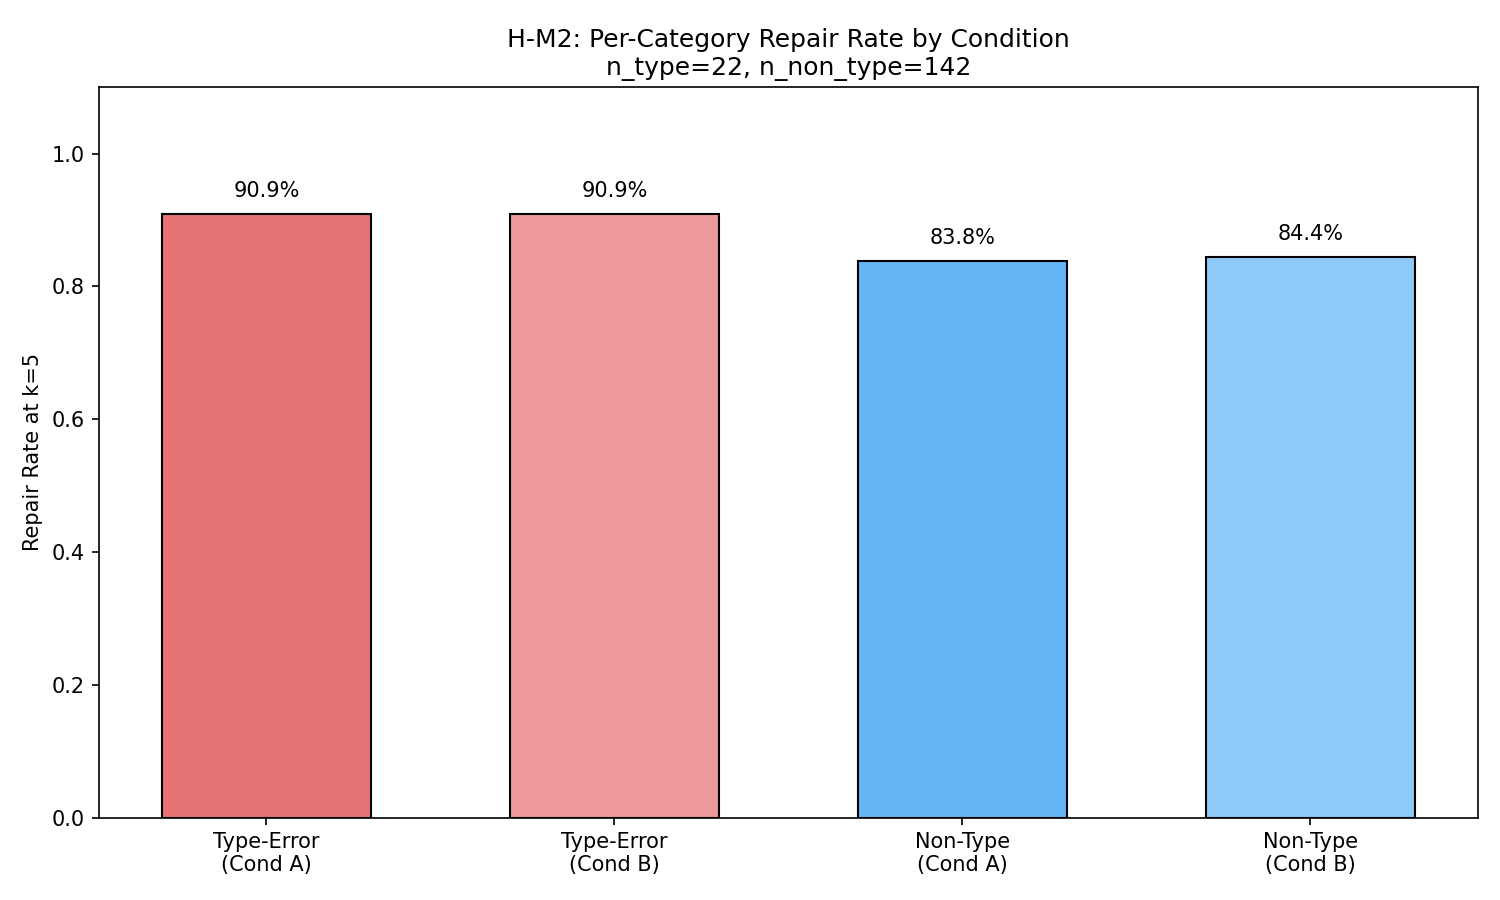
\includegraphics[width=0.9\columnwidth]{figures/repair_rate_comparison.png}
\caption{Repair rates for type-error and non-type-error problems under
Conditions A and B.}
\label{fig:repair_rate}
\end{figure}

\begin{figure}[h]
\centering
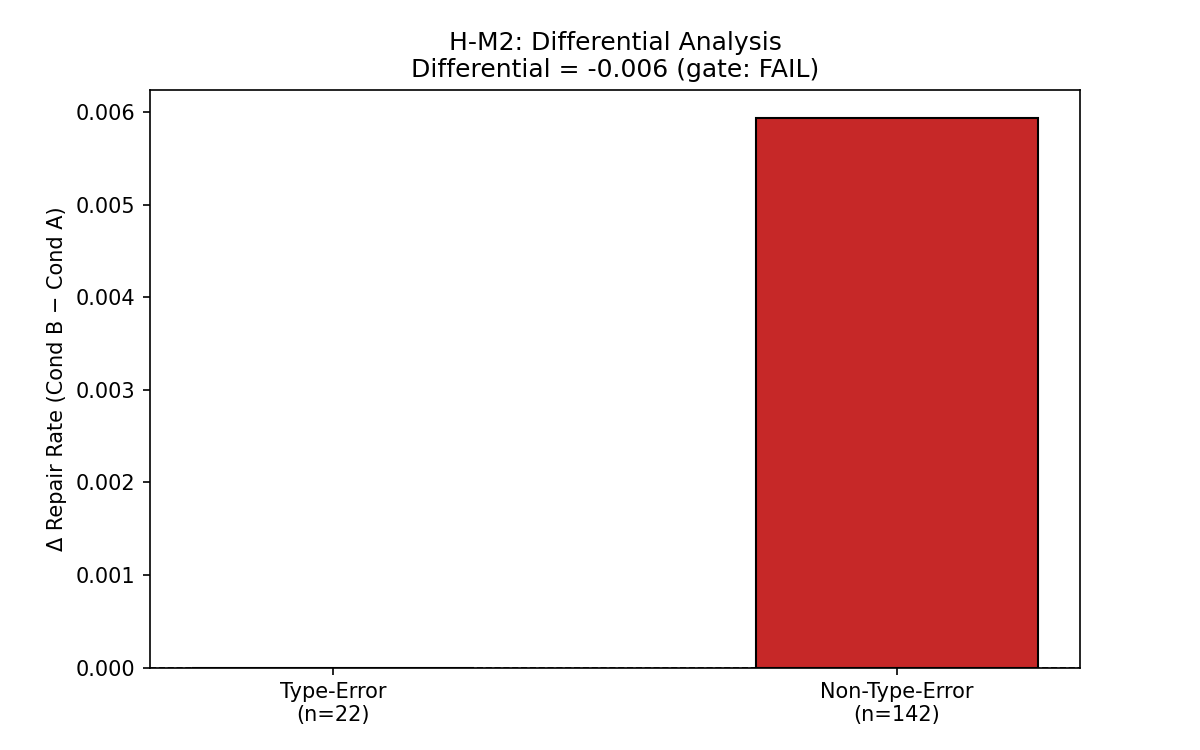
\includegraphics[width=0.9\columnwidth]{figures/differential_chart.png}
\caption{Type-specificity differential chart.}
\label{fig:differential}
\end{figure}

\emph{Interpretation:} The type-specificity mechanism is not active at $k$=5
saturation. Type-error problems reach a 90.9\% ceiling under execution-only
repair; mypy adds no further improvement for these problems. The overall
improvement must arise from a different mechanism --- most plausibly general
context enrichment.

\subsection{RQ4: Overall Pass@1 Comparison (h-m3)}

\begin{table}[h]
\centering
\caption{pass@1 on HumanEval+ (164 problems, GPT-4o-mini, $k$=5 rounds).}
\label{tab:pass1}
\begin{tabular}{@{}llll@{}}
\toprule
Seed & Cond.\ A & Cond.\ B & Delta \\
\midrule
42 & 79.9\% & 86.6\% & +6.7pp \\
123 & 76.8\% & 87.8\% & +11.0pp \\
456 & 78.1\% & 87.2\% & +9.2pp \\
\midrule
\textbf{Mean} & \textbf{78.25\%} & \textbf{87.20\%} & \textbf{+8.94pp} \\
\bottomrule
\end{tabular}
\end{table}

Execution+mypy repair achieves \textbf{87.20\% pass@1} versus \textbf{78.25\%}
for execution-only --- a \textbf{+8.94pp} improvement (seed std: A = $\pm$1.56pp,
B = $\pm$0.49pp; delta range: 6.7pp to 11.0pp). The direction is consistent
across all three seeds (no seed shows A $\geq$ B).

\emph{Interpretation:} This is the primary empirical contribution. The
improvement is real, reproducible, and substantial. Combined with the RQ3 null
result, this establishes that mypy improves repair quality broadly --- through
general diagnostic context enrichment rather than type-targeted correction.

\subsection{RQ5: Z3 Counterexample Feedback (h-z1)}

Figure~\ref{fig:z3_funnel} shows the Z3 pipeline funnel.

\begin{figure}[h]
\centering
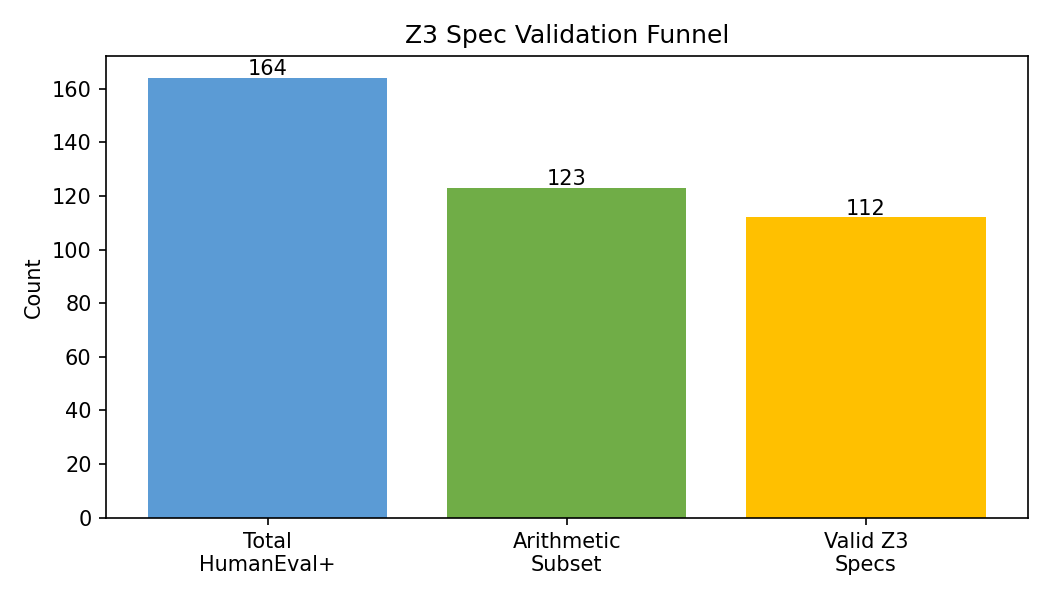
\includegraphics[width=0.9\columnwidth]{figures/z3_funnel.png}
\caption{Z3 validation funnel: 123 arithmetic problems $\to$ 112 valid specs
(91.1\%) $\to$ 18 problems with $\geq$1 counterexample (16.1\% CE rate).}
\label{fig:z3_funnel}
\end{figure}

\begin{figure}[h]
\centering
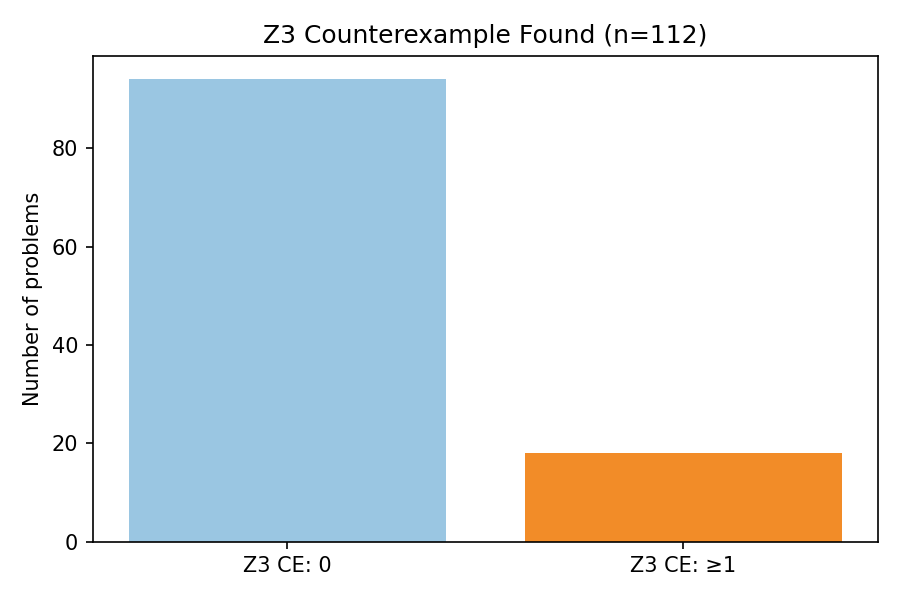
\includegraphics[width=0.9\columnwidth]{figures/z3_ce_distribution.png}
\caption{Z3 counterexample found vs.\ not found by problem.}
\label{fig:z3_ce}
\end{figure}

\begin{table}[h]
\centering
\caption{pass@1 on arithmetic subset ($n$=112, valid Z3 specs, seed=42, $k$=5).}
\label{tab:z3}
\begin{tabular}{@{}ll@{}}
\toprule
Condition & pass@1 \\
\midrule
B (execution+mypy) & 86.6\% \\
C (execution+mypy+Z3) & 85.7\% \\
Delta (C $-$ B) & \textbf{$-$0.9pp} \\
\bottomrule
\end{tabular}
\end{table}

\begin{figure}[h]
\centering
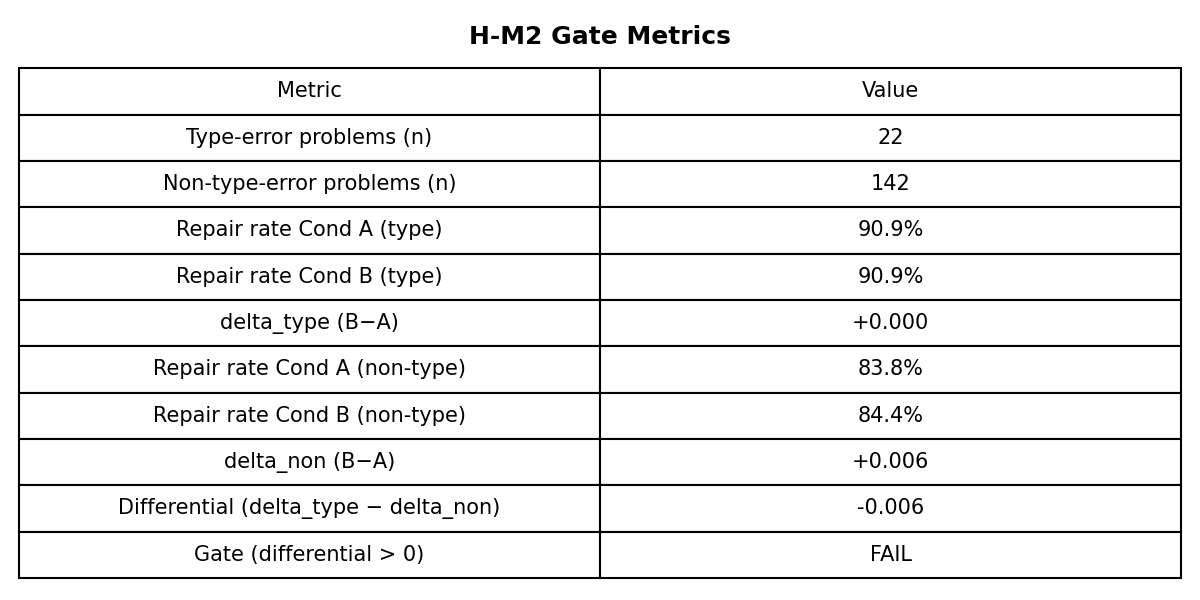
\includegraphics[width=0.9\columnwidth]{figures/gate_metrics.png}
\caption{pass@1 comparison between Conditions B and C on the arithmetic subset.}
\label{fig:gate_metrics}
\end{figure}

\emph{Interpretation:} Z3 CE feedback does not improve pass@1 beyond
execution+mypy. Two factors explain this: CE activation rate is low (16.1\%)
and base pass@1 (86.6\%) leaves only 13.4\% headroom. The Z3 pipeline's
primary contribution is the 91.1\% spec validity rate, establishing feasibility
for future work on harder problems with more headroom.

\subsection{Summary}

\begin{table}[h]
\centering
\caption{Summary of sub-hypothesis outcomes.}
\label{tab:summary}
\begin{tabular}{@{}lllll@{}}
\toprule
RQ & Hyp. & Finding & Gate \\
\midrule
RQ1 & h-e1 & 70\% HumanEval+; 0\% MBPP+ & PASS \\
RQ2 & h-m1 & 1.55$\to$0.00; $\rho$=$-$0.707 & PASS \\
RQ3 & h-m2 & Differential=0.000 & FAIL (SHOULD) \\
RQ4 & h-m3 & +8.94pp, 3 seeds consistent & PASS \\
RQ5 & h-z1 & $-$0.9pp; CE=16.1\%; ceiling & FAIL (SHOULD) \\
\bottomrule
\end{tabular}
\end{table}

\section{Discussion}

\subsection{Key Findings}

\textbf{mypy augmentation provides substantial but mechanism-agnostic benefit.}
Our primary finding is a +8.94pp pass@1 improvement from adding mypy to
execution-based repair loops on HumanEval+ (GPT-4o-mini, $k$=5, three seeds
consistent). The type-specificity hypothesis --- that mypy helps specifically
for type-error problems --- is not supported. Both conditions achieve identical
90.9\% repair rates on type-error problems (h-m2, $n$=22, differential=0.000).
The most parsimonious interpretation --- pending ablation confirmation (see L2)
--- is \emph{general diagnostic context enrichment}: mypy output adds structured
text to the repair prompt that may activate GPT-4o-mini's latent knowledge about
Python error patterns, improving repair quality across problem types. This
suggests that other structured diagnostic channels (linters, semantic analyzers)
might provide similar benefits, independent of whether they target the specific
failure mode.

\textbf{Benchmark-level signal divergence changes the applicability picture.}
The 70\% vs 0\% mypy error rate between HumanEval+ and MBPP+ is a new empirical
finding. HumanEval+ failures are dominated by undefined-name errors; MBPP+
failures appear to be pure algorithmic correctness errors invisible to mypy.
This divergence provides a practical guideline: a practitioner should first
profile the mypy error rate in failing solutions before adding mypy feedback ---
if it is low ($<$10\%), mypy will not activate frequently enough to drive
improvement.

\textbf{Z3 counterexample feedback: sound architecture, insufficient activation.}
The Z3 null result ($-$0.9pp) is informative: the spec generation pipeline
achieves 91.1\% validity, confirming LLM-generated Z3 specs are mostly correct
on arithmetic HumanEval+ problems. The bottleneck is CE activation (16.1\%).
Z3 counterexamples would be most valuable on problems where base pass@1 is
well below the ceiling ($<$60\%), leaving genuine headroom for guided repair.

\subsection{Limitations}

\textbf{L1: MBPP+ pass@1 comparison not completed.} All quantitative pass@1
claims (+8.94pp) are HumanEval+-specific. The h-m3 MBPP+ experiment was started
(122/378 tasks, seed=42, Condition A only) but not completed due to compute
constraints. Given the 0\% mypy error rate on MBPP+ (h-e1, h-m1), Condition B
is unlikely to show improvement on MBPP+ --- but this remains unconfirmed. We
restrict all pass@1 claims to HumanEval+.

\textbf{L2: Type-specificity mechanism alternative unverified.} We propose
general context enrichment as the active mechanism, but the ablation study
needed to confirm it (Condition B-Null: same prompt length as B, but with
generic filler text instead of mypy output) was not executed. Without this
ablation, we cannot distinguish mypy \emph{content} from mypy \emph{length} as
the active ingredient. This is the highest-priority future experiment.

\textbf{L3: Single model (GPT-4o-mini).} The repair benefit may be
model-capability-dependent. Replication with at least one open-source code
model is straightforward future work.

\textbf{L4: Z3 feedback at high base pass@1.} The arithmetic subset experiment
was conducted at base pass@1\_B = 86.6\%, leaving 13.4\% headroom. The null
result may not generalize to settings with lower base pass@1.

\subsection{Broader Impact}

This work establishes that adding mypy to LLM repair loops provides substantial,
reproducible improvement in Python code generation quality. Practical deployment
is low-cost (one subprocess call per repair round, ${\sim}$30ms latency). The
finding that the improvement is not type-specific suggests that other structured
feedback channels deserve controlled experimental evaluation rather than being
bundled with execution feedback and assumed beneficial. The Z3 pipeline
(91.1\% valid specs) establishes feasibility for automated formal specification
generation, a building block for future formal verification of LLM-generated
code. We do not foresee significant negative impacts: improving automated repair
quality does not introduce new failure modes beyond those of LLM-generated code
generally.

\section{Conclusion}

We set out to test whether adding mypy to LLM repair loops improves pass@1.
It does --- by nearly 9 percentage points, consistently across three seeds. We
also set out to understand why. The answer surprised us: the improvement is
not where we expected it.

The type-specificity mechanism --- mypy identifies a type error, tells the LLM
exactly what went wrong, the LLM corrects it specifically --- turns out not to
be the active channel at $k$=5 saturation. Both conditions achieve identical
90.9\% repair rates on type-error problems. The +8.94pp overall improvement
arises elsewhere, most plausibly from general diagnostic context enrichment:
mypy output adds structured text to repair prompts that improves GPT-4o-mini's
repair quality across all problem types.

Our contributions are: (1) first controlled evidence that execution+mypy
outperforms execution-only repair on HumanEval+ (+8.94pp, three seeds
consistent); (2) pre-registered type-specificity refutation
(differential=0.000, $n$=22); (3) benchmark-level mypy signal characterization
(70\% vs 0\%); and (4) Z3 spec generation pipeline (91.1\% validity). Together,
these results establish both the \emph{what} (mypy helps substantially) and the
\emph{what not} (not via type-targeted correction), opening a research agenda
about what makes feedback signals distinctive from execution output.

\textbf{Future directions} include: (a) Condition B-Null ablation to distinguish
mypy content from prompt length effects (highest priority); (b) per-round
type-specificity analysis at $k$=1..2 before ceiling saturation; (c)
multi-model replication (GPT-4o, open-source code models); and (d) Z3 CE
feedback on harder benchmarks (LiveCodeBench) with lower base pass@1 and more
headroom.

We began by asking whether adding mypy was worth the one-subprocess-call
investment. The answer is yes. The research question that emerged is richer:
\emph{why} does mypy help, and where does its benefit concentrate?
Understanding what makes a feedback signal distinctive from execution output ---
whether it is error specificity, structured format, or prompt enrichment --- is
the key to principled design of LLM repair loop architectures.


% ============================================================================
% REFERENCES
% ============================================================================

\bibliography{references}
\IfFileExists{icml2025.sty}{
  \bibliographystyle{icml2025}
}{
  \bibliographystyle{plainnat}
}

% ============================================================================
% APPENDIX
% ============================================================================

\newpage
\appendix
\section*{Appendix}

\subsection*{A. Additional Figures}

\begin{figure}[h]
\centering
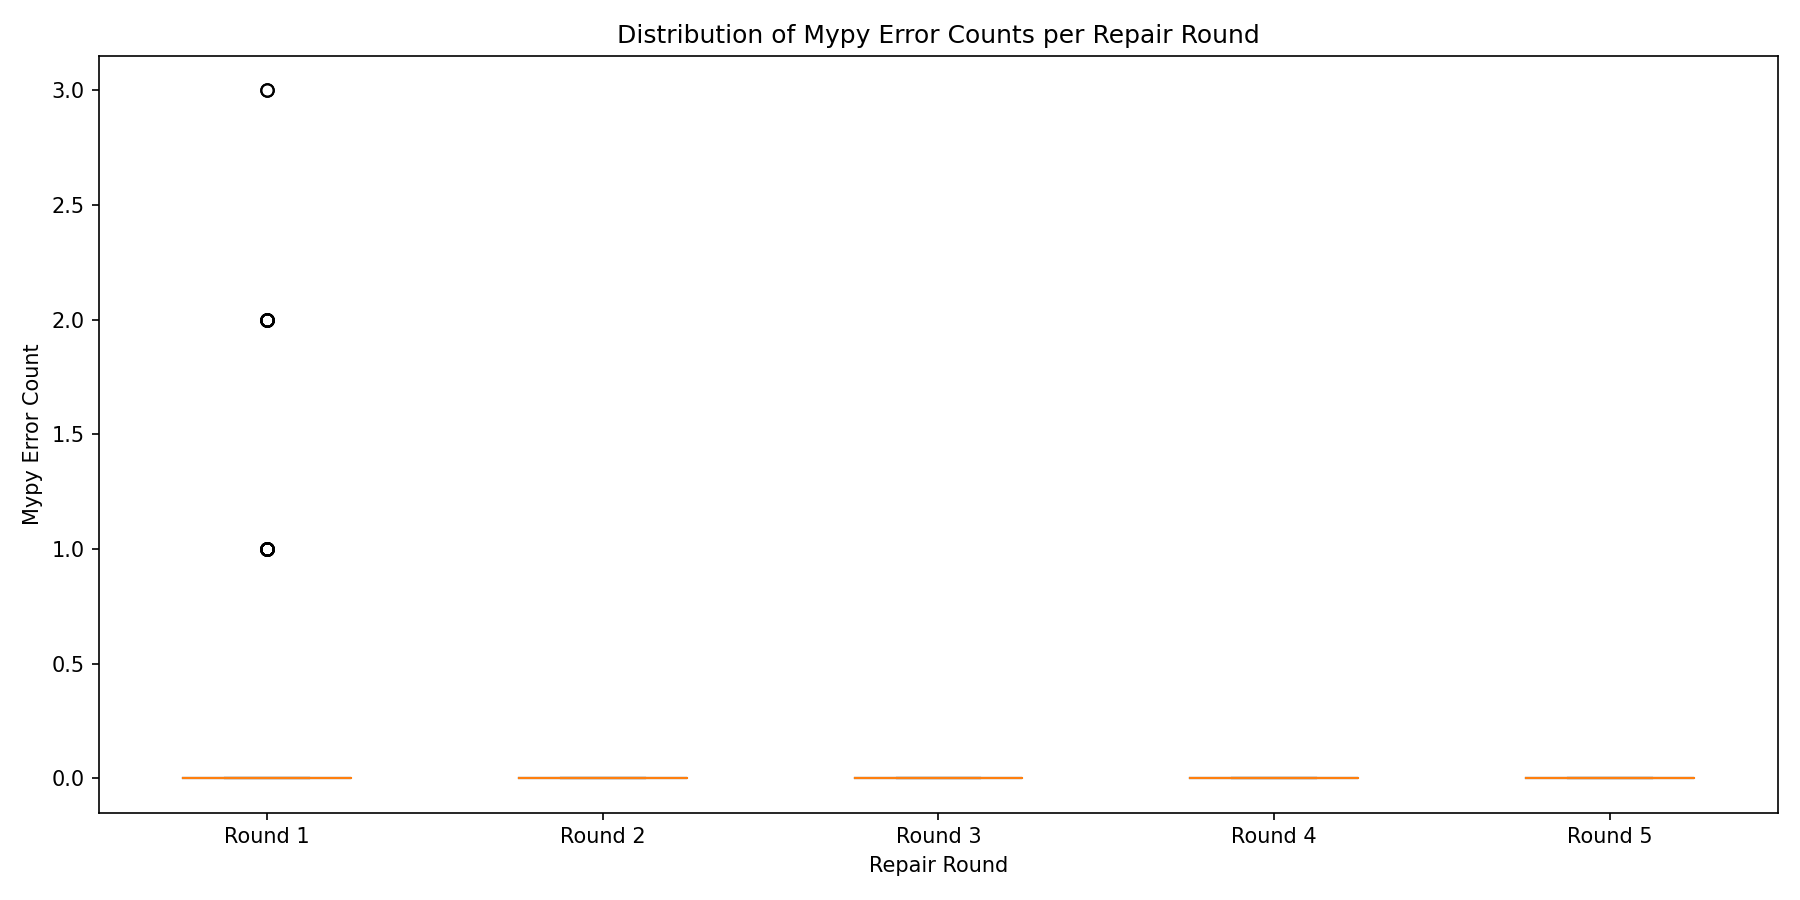
\includegraphics[width=0.9\columnwidth]{figures/error_distribution.png}
\caption{Distribution of mypy error counts across HumanEval+ failing solutions.}
\label{fig:error_distribution}
\end{figure}

\begin{figure}[h]
\centering
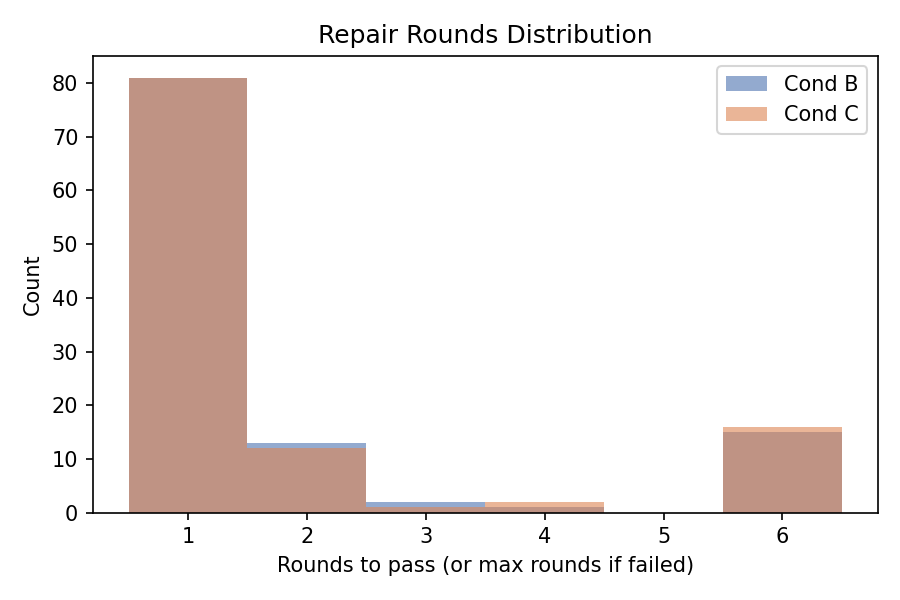
\includegraphics[width=0.9\columnwidth]{figures/repair_rounds.png}
\caption{Pass@1 by repair round for Conditions A and B on HumanEval+.}
\label{fig:repair_rounds}
\end{figure}

\begin{figure}[h]
\centering
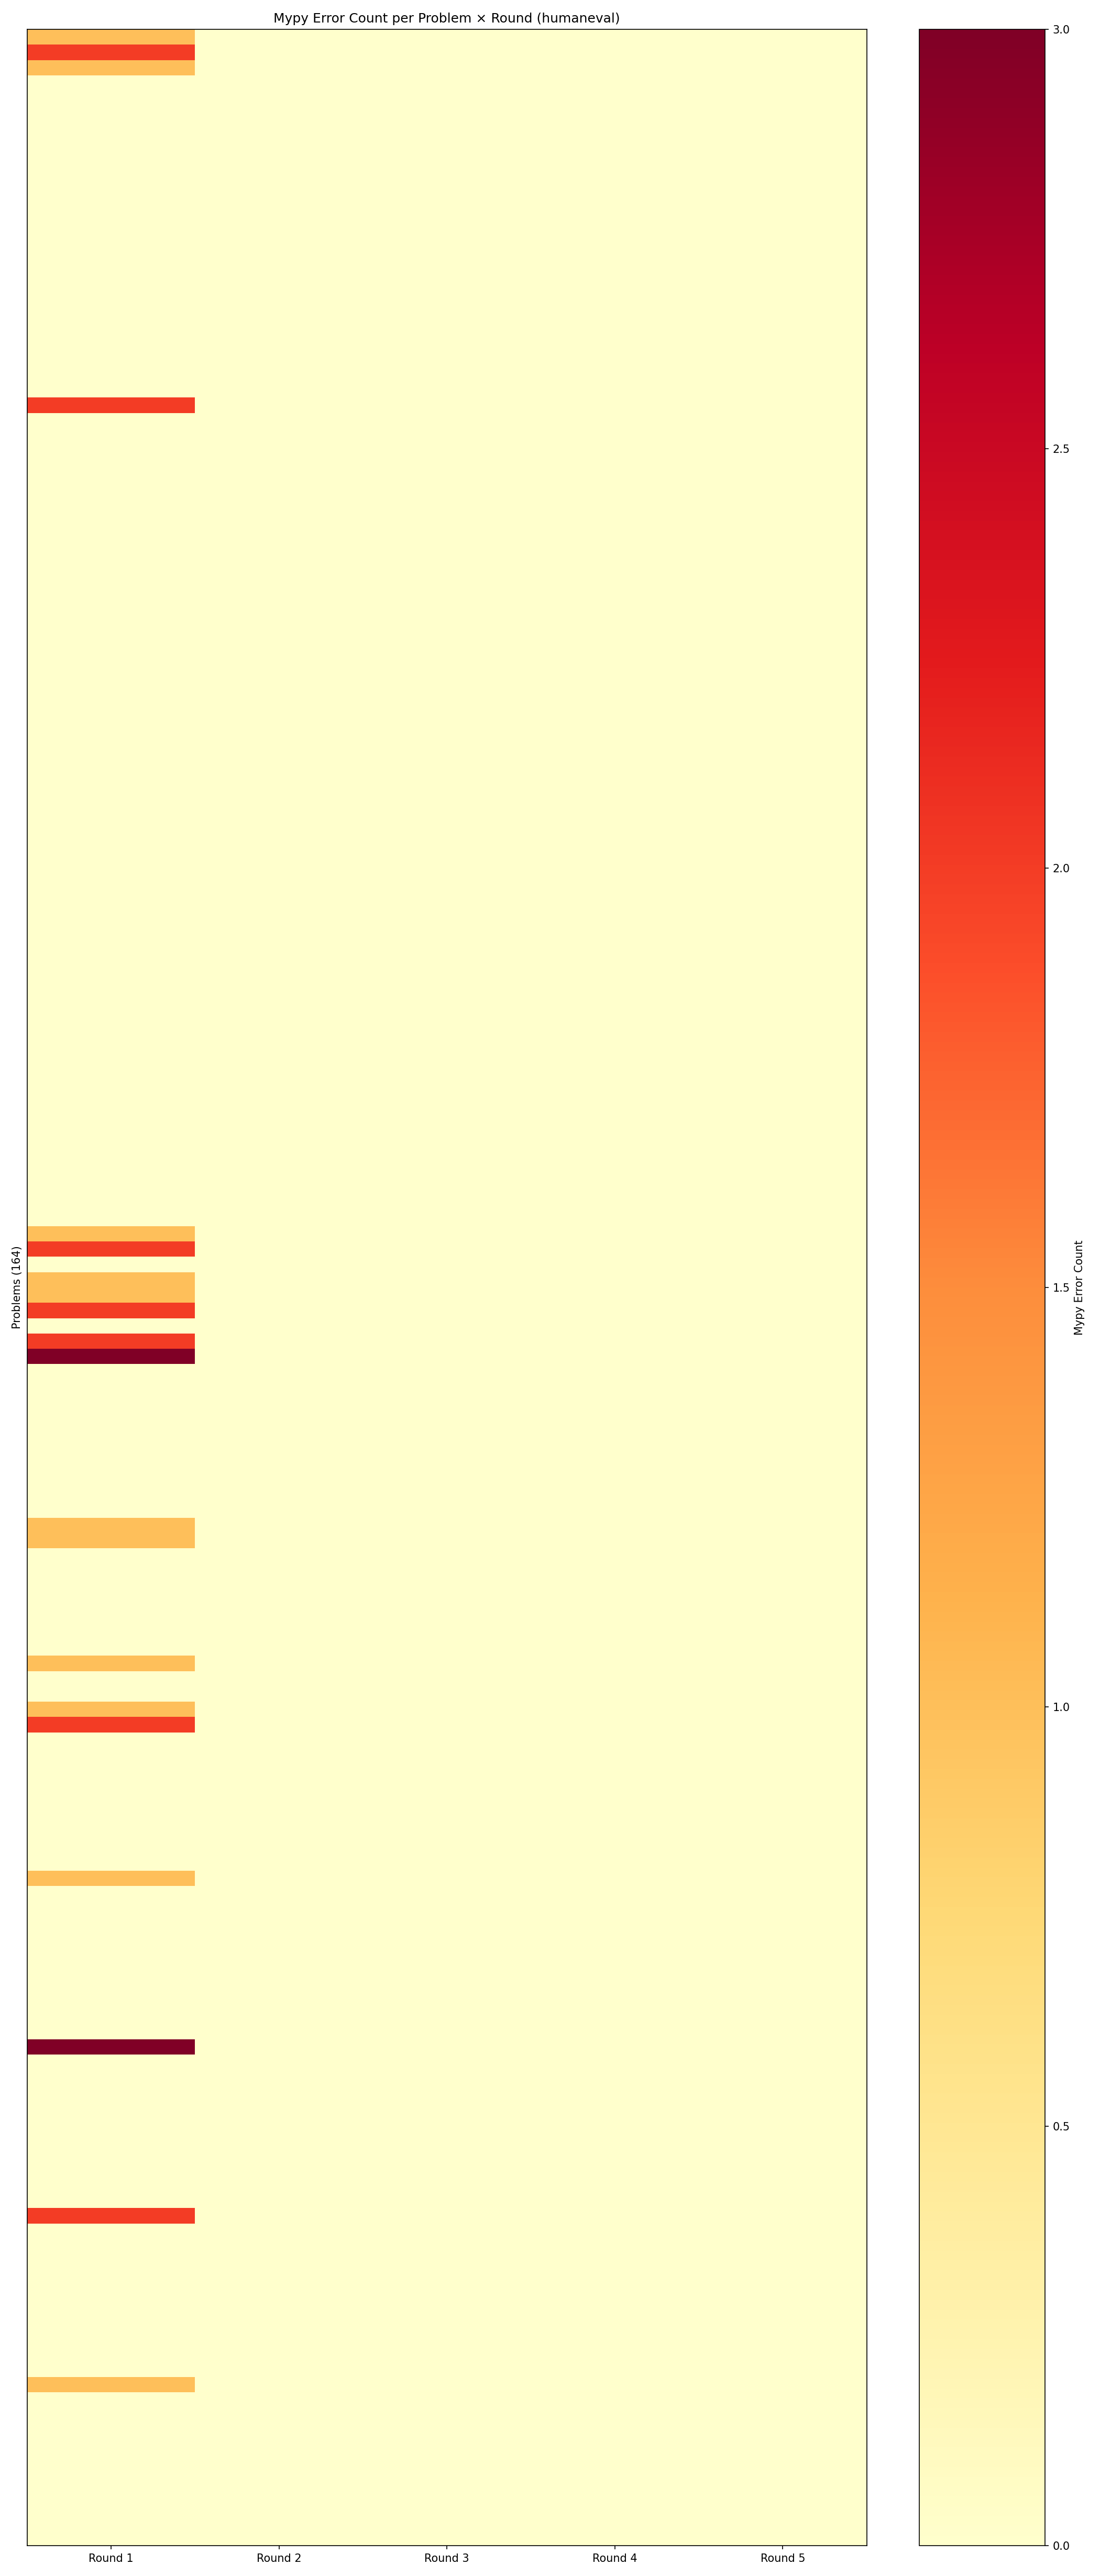
\includegraphics[width=0.9\columnwidth]{figures/heatmap_humaneval.png}
\caption{Per-problem pass/fail heatmap for Conditions A and B across seeds
on HumanEval+.}
\label{fig:heatmap}
\end{figure}

\subsection*{B. Implementation Notes}

All code is implemented in Python 3.10. The repair loop harness makes
sequential API calls to GPT-4o-mini with exponential backoff on rate-limit
errors. mypy is invoked as a subprocess with a 30-second timeout per call.
Z3 (version 4.12) is invoked via the \texttt{z3-solver} Python package.
EvalPlus version 0.2.0 is used for test harness evaluation. All experiments
were run on a single machine with 32GB RAM; wall-clock time for the full
HumanEval+ experiment (3 seeds, 2 conditions) was approximately 6 hours.

\subsection*{C. Prompt Templates}

The repair prompt for Condition B follows this structure:

\begin{verbatim}
System: You are a Python expert. Fix the following code.

Problem: {problem_description}

Current solution:
```python
{current_solution}
```

Execution feedback:
{execution_feedback}

mypy output:
{mypy_output}

Provide the corrected complete Python function.
\end{verbatim}

Condition A omits the ``mypy output'' block. Condition C adds a ``Z3
counterexample'' block after the mypy output block.


\end{document}
